\documentclass[twocolumn, 10pt, a4paper]{article}

% standard packages
\usepackage{titlesec, blindtext, color,multicol,multirow,url}   % standard packages
\usepackage[usenames,dvipsnames,svgnames,table]{xcolor} % extra colors 
\usepackage{graphicx}                                                       % figures
\usepackage{natbib}                                                          % bibliography
\usepackage[english]{babel}                                               % correct hyphenation (afbreekstreepjes)
\usepackage{booktabs}                                                      % for midrule in tables
\usepackage{rotating}                                                        % for sdeways table
\usepackage{amssymb}                                                     % more symbols
\usepackage{arydshln}                                                       % for dashed lines in tables
\usepackage{fancybox}                                                      % for environments
%\usepackage{fvrb-ex}                                                         % for environments
\usepackage{multido}                                                        % for environments
%\usepackage{boxedminipage}                                             % package for making question boxes


%%%%%%%%%%%%%%%%%%%%%%%%%%%%%%

% PAGE MARGINS
\usepackage[top=2cm, bottom=2.5cm, left=1.6cm, right=1.6cm]{geometry}

% FONT
\usepackage[lf]{berenis}
\renewcommand*\familydefault{\sfdefault} 
\usepackage[T1]{fontenc}
% for other fonts, and how to install them, see the LaTeX Font Catalogue:
% http://www.tug.dk/FontCatalogue/
\definecolor{light-gray}{gray}{0.75}

% LINE SPACE
\linespread{1.1}                          % more space between lines
\setlength{\parindent}{5mm}       % indenting first line paragraph

% FOOTNOTES
\renewcommand{\thefootnote}{\fnsymbol{footnote}} 
% sets the footnotesymbols to fn in stead of numbers

% OTHER
\renewcommand{\floatpagefraction}{.8}   % to prevent figures from becoming full-page

%%%%%%%%%%%%%%%%%%%%%%%%%%%%%%

% The environment for practical-style questions
\definecolor{light-gray}{gray}{0.85}
\newenvironment{PC_prac_environment}{
% Q for begin question
\def\Q{\noindent \color{Gray}\rule[-0.1cm]{\columnwidth}{1.5pt}  \color{black} } \let\ques\Q 
% nQ for next question (without starting line)
\def\nQ{\noindent \color{black} } \let\ques\nQ 
% \E for end
\def\E{\color{Gray}\rule[0.3cm]{\columnwidth}{1.5pt} \color{black}} \let\ques\E }

%%% show answers or show lines 
\newboolean{showanswer} \setboolean{showanswer}{false} % <-- CHANGE HERE FOR LINES/ANSWERS
\newcommand{\A}[2] { \ifthenelse{\boolean{showanswer}} {\noindent \color{cyan}{#2}\color{black}} {\multido{}{#1}{\noindent \color{light-gray}\hrulefill\\} } }

%%%%%%%%%%%%%%%%%%%%%%%%%%%%%%%%%%%%%%%%%%%%%%%%
%%%%%%%%%%%%%%%%%%%%%%%%%%%%%%%%%%%%%%%%%%%%%%%%
%%%%%%%%%%%%%%%%%%%%%%%%%%%%%%%%%%%%%%%%%%%%%%%%

%CHANGE "showanswer" TO "false" OR "true" FOR DIFFERENT VERSIONS (8 LINES ABOVE THIS ONE)


\title{\vspace{-1.4cm} 
\huge{\textbf{Topography based models}}\\
\Large{\textbf{PC practical Catchment and Climate Hydrology}}}
\date{\vspace{-1cm}}


\begin{document}
\begin{PC_prac_environment}
\maketitle

\section{Introduction}
This practical focuses on the importance of the catchment geomorphology for the catchment response to rainfall. Digital elevation models (DEMs) are relatively easily available (compared to e.g. soil maps or the location of river branches) and are often used as a first tool to characterize catchments. A detailed analysis of a digital elevation model will give a first idea of how the discharge will respond to rainfall events. 

You don't have to do all exercises, but make sure you start with the Sec.~5 at approximately 11:30, Sec.~6 at 12:00 and the final assignment at 12:30. We discuss the results at 13.05.

\section{The Ourthe catchment}
We will focus specifically on the catchment of the Ourthe upstream of Tabreux (1600~km$^2$). Both topography and geomorphology play an important role in the hydrological response of the Upper Ourthe catchment. The catchment is situated in the hilly plateaus of the Ardennes in the eastern part of Belgium\footnote{a well-known area for those who followed Hydrogeology} (Figure \ref{fig:f1}). The elevation of the catchment varies between 150 and 650~m above sea level. The soil mainly consists of sandstone, shale and limestone, which have been eroded by small river systems that drain into the river Meuse. The region can be characterized as mostly rain-fed with some snow during the winter period. This results in a highly variable runoff regime with low discharges in summer and high peaks in winter. 

\begin{figure}
	\centering
	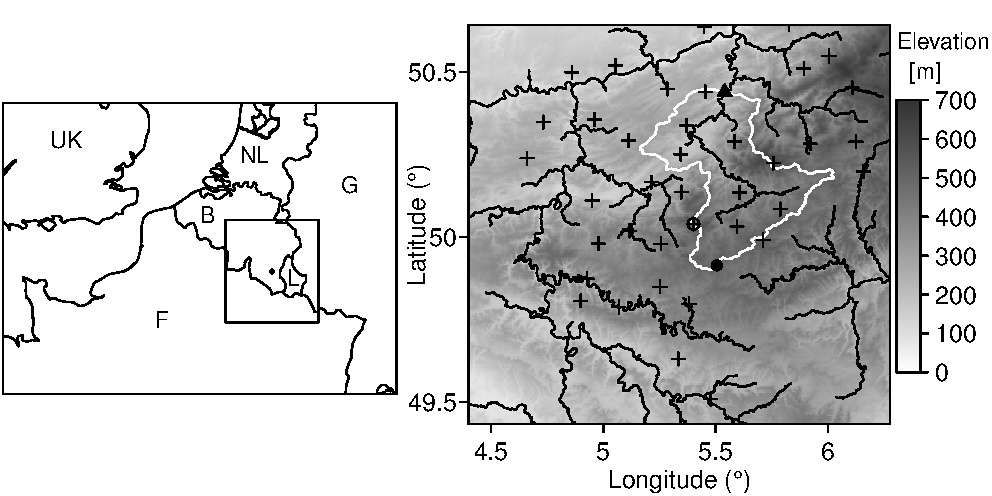
\includegraphics[width=.32\columnwidth, trim=0mm 15mm 100mm 0mm, clip=true]{topomap.pdf}
	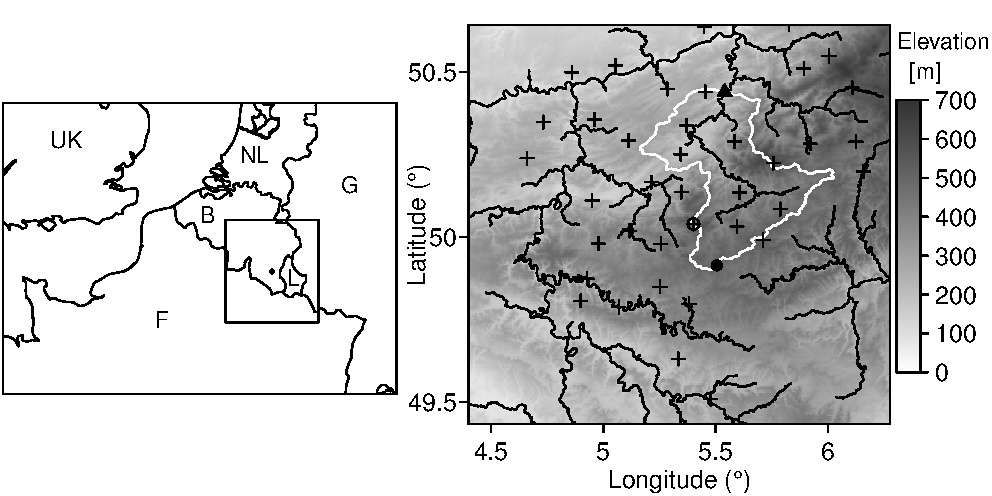
\includegraphics[width=.8\columnwidth, trim=68mm 0mm 0mm 0mm, clip=true]{topomap.pdf}
	\caption{Location of the Ardennes and a 200x200-km box with a topographic map, the main channel network (black), the Ourthe catchment boundary (white), the catchment outlet ($\blacktriangle$), the meteorological station ($\circ$), rain gauges (+) and weather radar ($\bullet$).}
	\label{fig:f1}
\end{figure}

\section{Digital elevation models for hydrological applications}
The data and scripts can be found on Brightspace. Download and unzip. This will generate the folder \verb!topmodels!, containing the subdirectories \verb!R_scripts!, \texttt{DEM} and \texttt{Data}. 

\subsection{DEM}
The DEM you will use today was obtained by the Shuttle Radar Topography Mission (SRTM) which generated a near global elevation map. For Europe the resolution of this dataset is about 90~meter and can be downloaded from the internet (\verb!http://www2.jpl.nasa.gov/srtm/!). Your DEM file is called \verb!ourthe_90m.asc! and is located in the folder \texttt{DEM}. 

\newpage
\Q Open this file in Notepad and find out how this ASCII file is set up. What do the numbers in the big matrix mean?\\
\A{1}{The elevation of each pixel.\\}
\E

\vspace{-0.5cm}
\subsection{Preprocessing}
Before you can use the DEM for hydrological applications, the DEM has to be preprocessed. In this preprocessing step, pits in the topography field are filled, flow directions are computed and contributing areas and slope gradients are computed.

For this preprocessing, multiple GIS programs can be used (e.g. ArcGIS, SAGA GIS, GRASS). For this practical these preprocessing steps have already been performed using the TAUDEM package. TAUDEM is a terrain analysis package for ArcGIS developed by D.G.~Tarboton of Utah State University. For more information concerning the specific aspects of TAUDEM, see \verb!http://hydrology.usu.edu/taudem/taudem5.0/! \verb!index.html!. The following sections explain what happens during the preprocessing phase.

\subsubsection{Sink / pit filling}
The main assumptions behind spatial hydrological analyses is that water will flow from higher to lower cells. To obtain a continuous flow direction map, the lowest cell in a DEM should be situated at the boundary of a DEM. Unfortunately, local topography or erroneous measurements by the satellite can result in local depressions (also called sinks or pits). Because the cells surrounding the pits are higher in elevation, water will never flow out of them and will never reach the river. 

Although sinks may represent real terrain features, they hinder the analysis of drainage networks. Local depressions should therefore be filled before making a flow direction map. Using TAUDEM, the original DEM file \verb!ourthe_90m.asc! was corrected for pits, resulting in a new DEM file \verb!ourthe_90mfel.asc!, which can also be found in the \texttt{DEM} folder.\\ 

\subsubsection{Flow direction, slope and contributing area}
There are many ways to compute flow directions. In this practical the simplest and oldest method will be applied: the D8 flow direction method. The elevation of each pixel is compared to the elevations of the 8~neighbouring cells and water will flow in the direction of the steepest descent:
\begin{center}
%\vspace{-0.3cm}
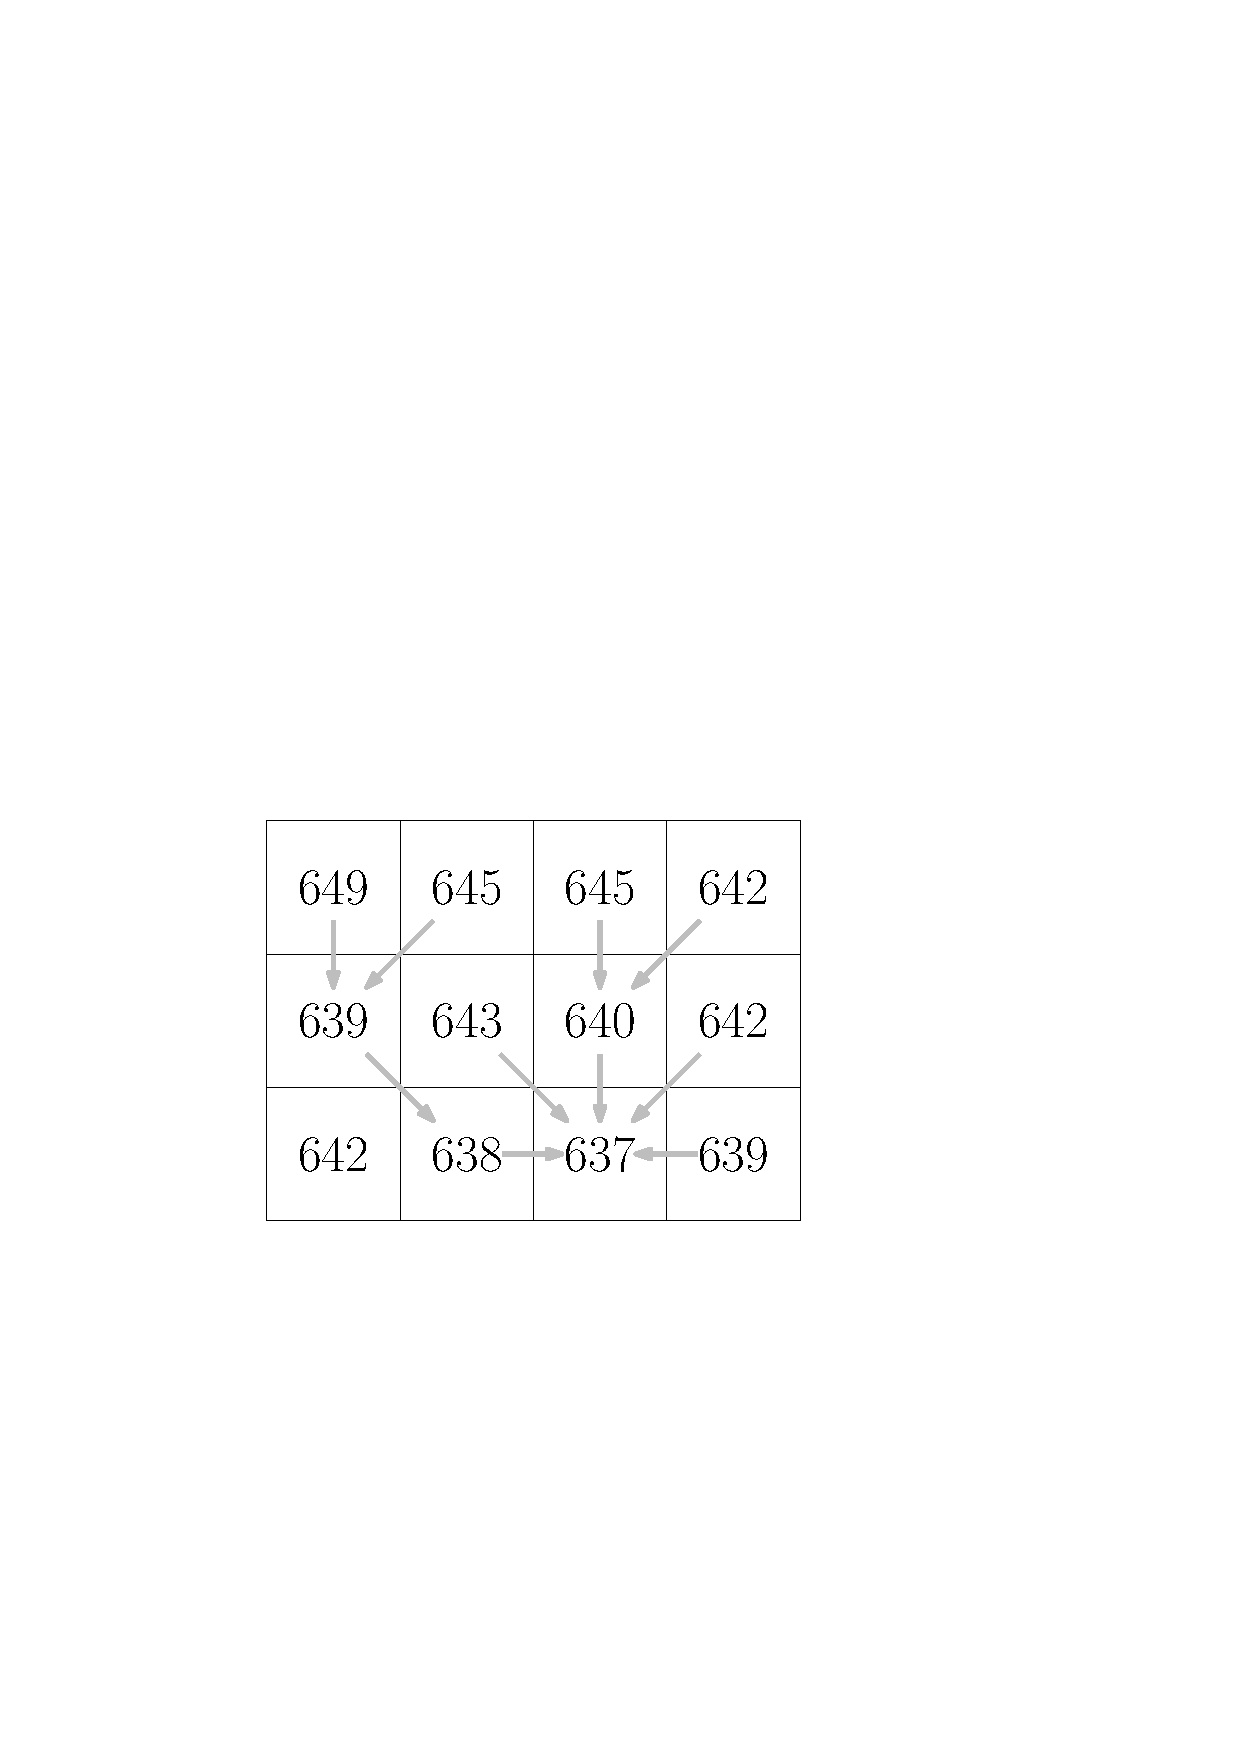
\includegraphics[width=0.31\columnwidth]{DEM_example.pdf}\\ 
%\vspace{-0.3cm}
\end{center}
The flow directions are represented by numbers:\\ 
\begin{center}
\vspace{-0.3cm}
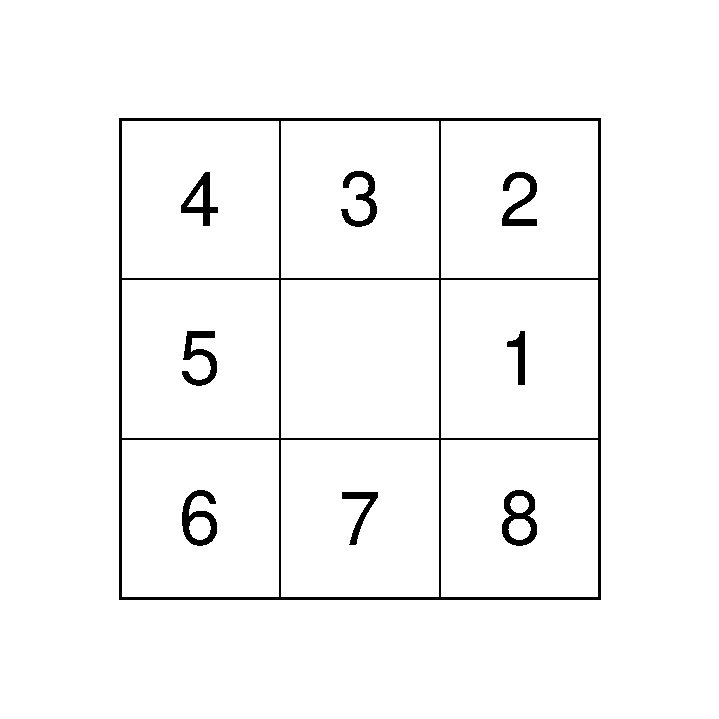
\includegraphics[width=0.16\columnwidth, trim=2cm 2cm 2cm 2cm,  clip=true]{D8_flow_directions.pdf} 
%\vspace{-0.3cm}
\end{center}
Boundary pixels for which no downstream direction could be obtained receive the value of $-1$. The output of this step was saved in the file \verb!ourthe_90mp.asc!. Once these directions have been determined, TAUDEM immediately generates the file \verb!ourthe_90msd8.asc!, containing the local slopes for all pixels. From the flow direction map, the upstream area for each pixel can be computed. TAUDEM starts at the highest points of the DEM and moves downward. In \verb!ourthe_90mad8.asc! the number of upstream pixels is given for each pixel.

\Q Open \verb!ourthe_90mp.asc!, \verb!ourthe_90msd8.asc! and \verb!ourthe_90mad8.asc! in Notepad and try to understand what the numbers mean.\\
\E


\subsection{R for DEM analyses}
After these preprocessing steps, R can be used for spatial hydrological analyses. Open RStudio and load the script \verb!topmodels.R!. Set the working directory and run the part under ``Getting started".

The folder \verb!R_scripts! contains more scripts with functions used in the main R script \verb!topmodels.R! (you don't have to open these scripts now):

\noindent\begin{tabular}{lp{7.8cm}}
$\bullet$&\texttt{SetGeo.R} gives pixel size and extent of the DEM.\\
$\bullet$&\texttt{nbrtable.R} Within R a DEM matrix is internally represented as a vector. Therefore, for every pixel within the grid this function calculates the vector index value for the 8 neighbour points.\\
\end{tabular}\\
\noindent\begin{tabular}{lp{7.8cm}}
$\bullet$&\texttt{downnbr.R} gives the vector index number of a pixel's downstream neighbour based on the D8 flow direction method.\\
$\bullet$&\texttt{mainbasin.R} gives the upstream area for a given pixel.\\
$\bullet$&\texttt{GetNewCoordinates.R} zooms in to the catchment when the catchment area covers a small part of the DEM.\\
$\bullet$&\texttt{flowdistance.R} calculates the distance to the channel network for each pixel.\\
$\bullet$&\texttt{plotflowdistance.R} draws a map of the distance to the channel for each pixel obtained by \texttt{flowdistance.R}.\\
$\bullet$&\texttt{channeldistance.R} gives the distance to the outlet (measured along the channel) for each pixel (given a certain channel network).\\
$\bullet$&\texttt{channelpixelsize.R} computes for each channel pixel how many metres of channel it contains.\\
$\bullet$&\texttt{strahler\_order.R} gives Strahler order numbers for each channel link.\\
$\bullet$&\texttt{shreve\_order.R} gives Shreve order numbers for each channel link.\\
$\bullet$&\texttt{TOPMODEL.R} runs the hydrological model TOPMODEL.\\
$\bullet$&\texttt{NSeff.R} computes the Nash-Sutcliffe efficiency.\\
\end{tabular}\\

%\newpage
Run the part under ``Extra functions''. You then load all extra functions. For example, when you run the line \verb!source("R_scripts/SetGeo.R")! in the \verb!topmodels.R!-script, R runs the whole \texttt{SetGeo.R}-script at once in the background. Because the \verb!SetGeo.R!-script contains the definition of the function \texttt{SetGeo}, this function with the argument \texttt{A} appears in the workspace window. 

\vspace{0.1cm}
\section{DEM analyses}

\subsection{Read data}
Next, run the part of the script under ``Read Data". This part of the script generates a map with the pit filled DEM. Check if your figure is similar to Figure \ref{fig:f1}.

Read the part of the script under ``Catchment Area". If you run this part in R, only the part of the DEM that lies upstream of Tabreux is selected. This part belongs to the Upper Ourthe catchment. 

\Q Click on \texttt{basin} in the workspace window. What do the TRUE and FALSE mean?\\
TRUE: \A{1}{Inside the catchment.\\}
FALSE: \A{1}{Outside the catchment.\\}
\E
Make sure you understand what happens in the line \texttt{Elevation[basin == FALSE] = NA}. If you don't know what the square brackets do, reread Section 11.1 of the (very) short introduction to R (which can be found on the R website: \texttt{cran.r-project.org/doc/contrib/} \texttt{Torfs+Brauer-Short-R-Intro.pdf}).

\Q How many pixels belong to the Ourthe catchment and what is the corresponding area?\\
\A{1}{The total number of pixels corresponding to the catchment is 199886, which corresponds to 1619 km$^{2}$.\\}
\E

\vspace{-3mm}
\subsection{Channel network}
\label{sec:channel_network}
Because you do not have information on where the channels are (which is almost always the case), you will predict the location of the channels with the DEM. Assume that a river branch will develop when the upstream area exceeds a certain value representing the soil's flow capacity; excess water will start to flow overland instead, creating a channel. Assume that for a pixel to be part of the channel network, the upstream area has to be equal to or exceed 0.1~km$^2$ ($A_c$). 

Run the part of the script under ``Channel Network". This will generate the channel network. Click on ``Channel'' in the workspace window to see what this matrix looks like.

\Q How many pixels are part of the channel network?\\
\A{1}{29177\\}
\nQ How many pixels are part of the network when you change the upstream area to 0.03, 0.3 and 1~$\mathrm{km}^2$.\\
0.03~$\mathrm{km}^2$: \A{1}{70973\\} 
0.3~$\mathrm{km}^2$: \A{1}{17288\\}
1~$\mathrm{km}^2$: \A{1}{10477\\}

\nQ What is the relation between channel density and $A_c$?\\
\A{1}{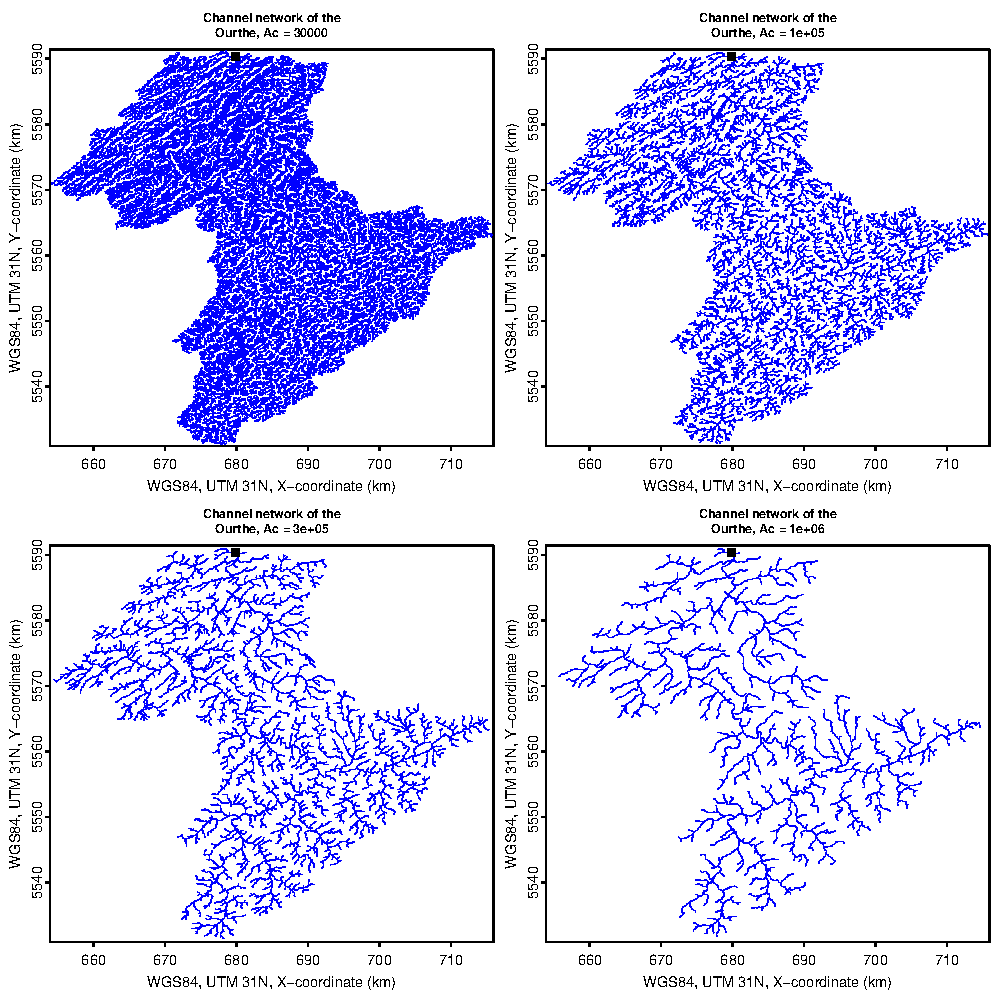
\includegraphics[width=\columnwidth]{Question3.pdf}
The channel density decreases when you increase Ac (the upstream area which should be exceeded in order to form a channel).\\}
\E
\noindent Set the upstream area to 0.1~km$^2$ for the next assignments.

\subsection{Channel network ordering}
The shape of channel network can be analyzed with several ordering systems. Today we will focus on the Strahler (left) and Shreve (right) ordering systems:

\hbox{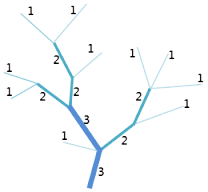
\includegraphics[width=0.5\columnwidth]{Strahler.png} 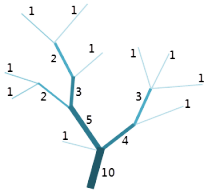
\includegraphics[width=0.5\columnwidth]{Shreve.png}}\vspace{4mm}
\noindent Use the function \texttt{shreve} to calculate the Shreve order for each channel pixel. 

\Q What is the maximum Shreve value? (Look at the arguments of the function \texttt{max} to find out how to exclude non-channel pixels in the computation.)\\
\A{1}{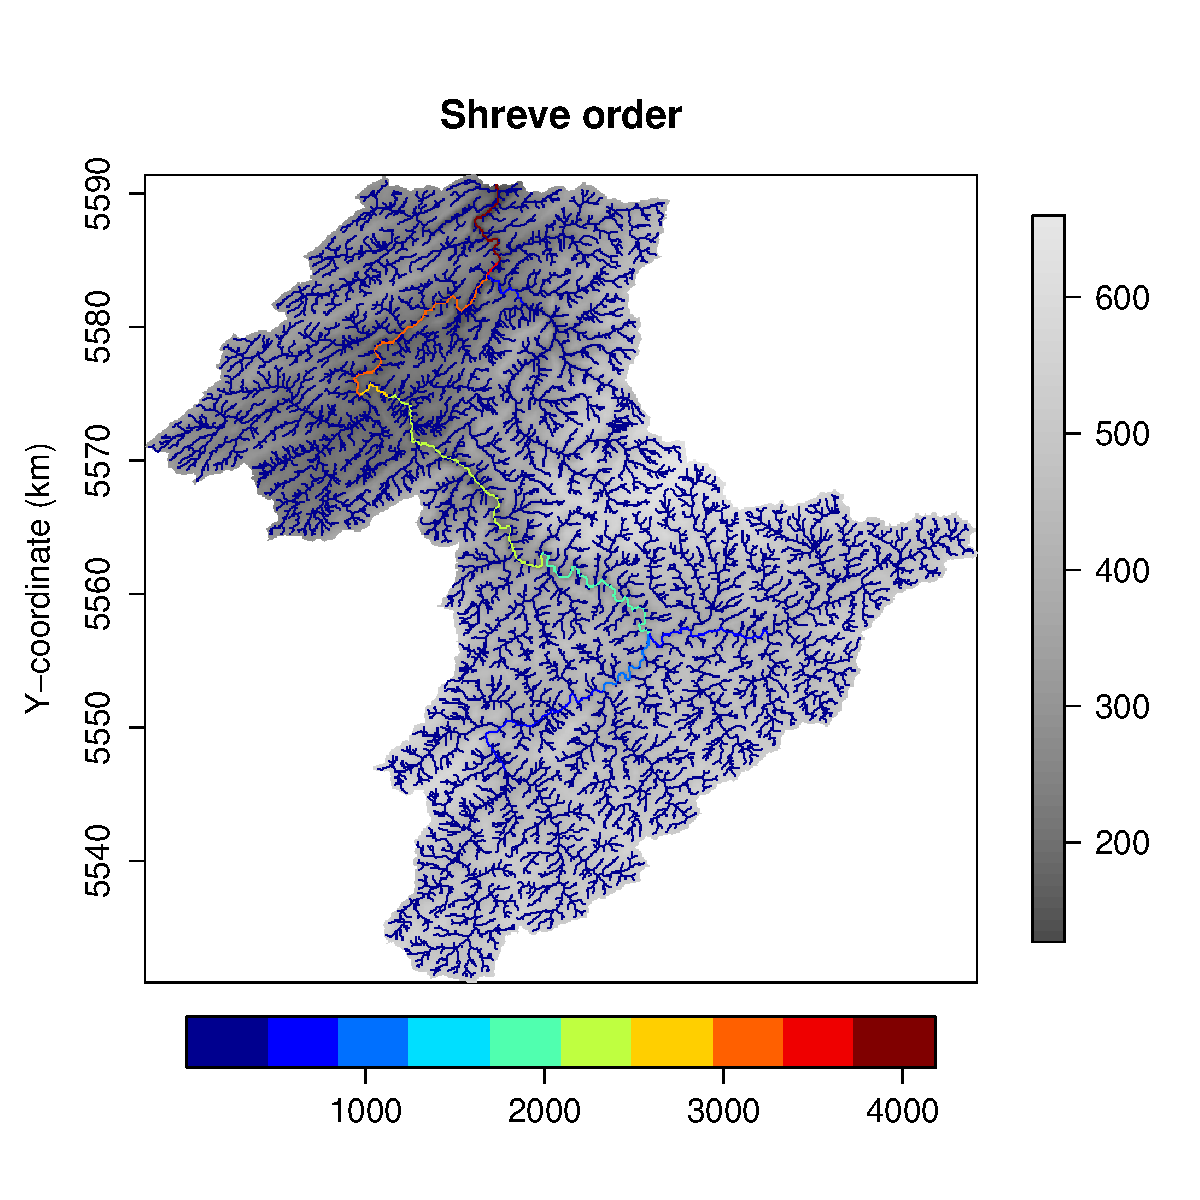
\includegraphics[width=\columnwidth]{Question11.pdf} 
4183\\}
\nQ What does this maximum represent? \\
\A{1}{This is the number of first order channels (and sources).\\}
\E
Do the same for the Strahler order.

\Q What is the maximum Strahler number?\\
\A{1}{7\\}
\nQ How does this value change when you increase $A_c$; the upstream area which defines the channel network? (what you did in section~\ref{sec:channel_network})\\
\A{2}{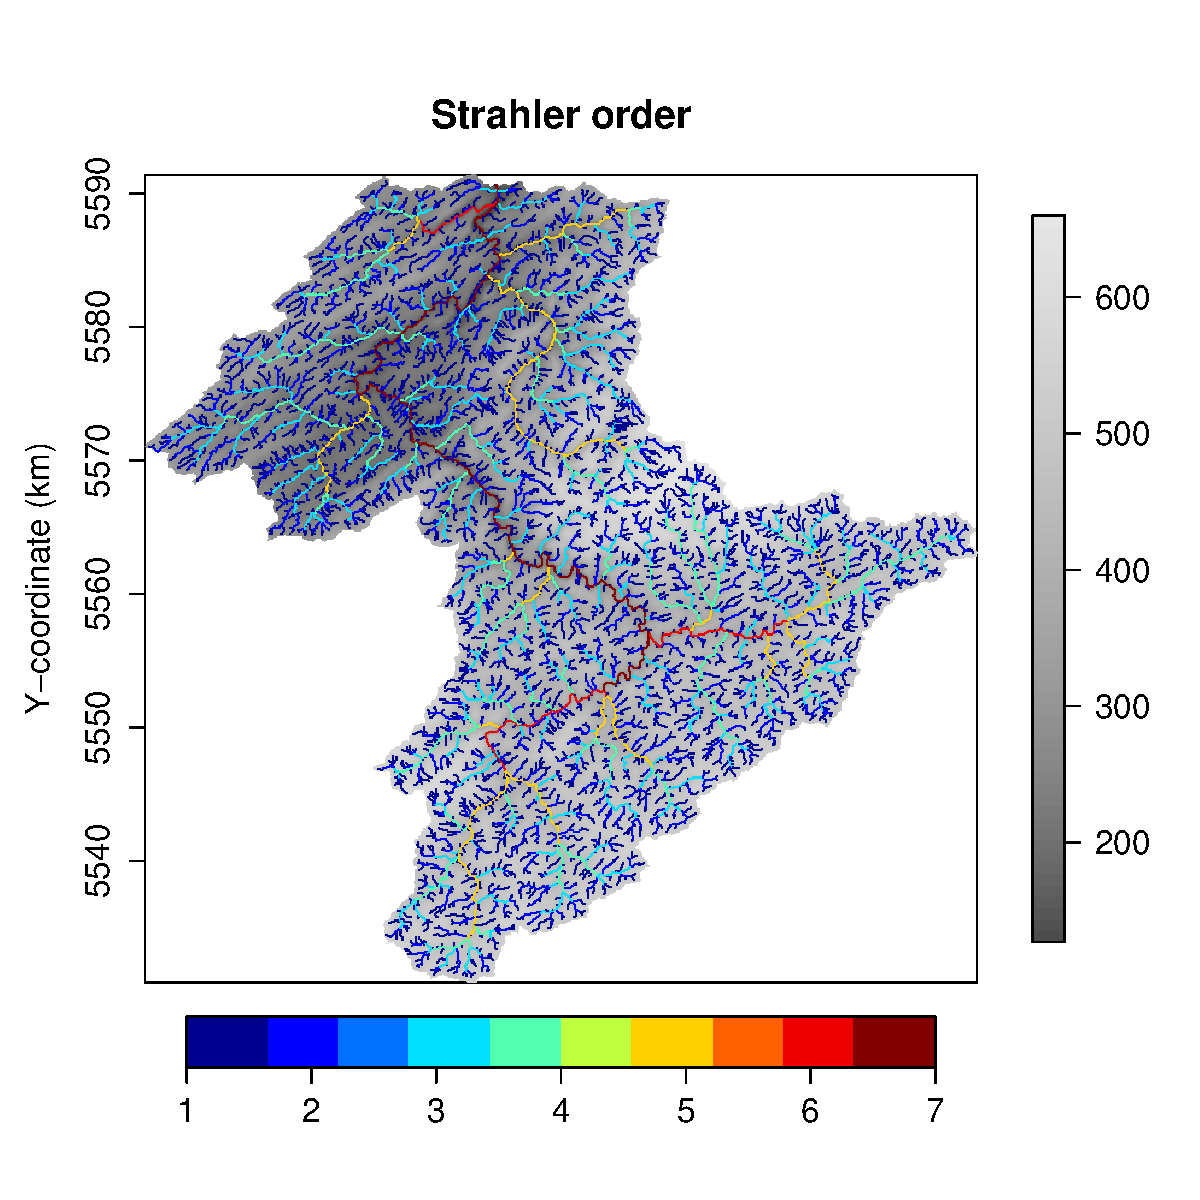
\includegraphics[width=\columnwidth]{Question12.pdf}
When the upstream area increases, the Strahler number will decrease, because there will be fewer branches.\\}
\E


\subsection{Drainage density and hillslope length}
\label{sec:dd}
The function \texttt{channelpixelsize} calculates for every channel pixel how many metres of channel it contains. 

\Q Click on \verb!Channel_Length_Per_Pixel! in the workspace window. What do NA, 90 and 127 tell you about the flow direction?\\
NA:\A{1}{There is no river on this pixel\\}
90:\A{1}{The river flows horizontally or vertically through this pixel.\\}
127:\A{1}{The river flows diagonally through this pixel.\\}
\nQ Where do the numbers 90 and 127 come from?\\
\A{1}{Size of the pixel is 90~m and $127 \sim \sqrt(90^2 + 90^2)$\\}
\E

A rectangular valley with a channel in the middle and the local water divide at the edges, can be characterized by several measures: the channel length $L_c$, the area $A$, the hillslope length $L_h$ and the drainage density $d$:\\

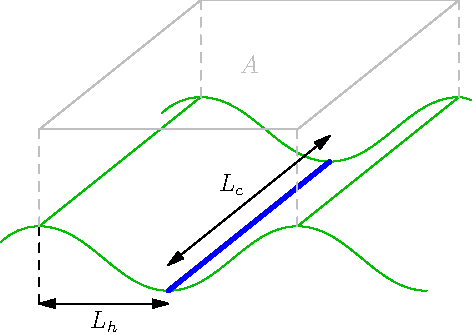
\includegraphics[width=0.75\columnwidth]{hillslope.pdf}\\\vspace{2mm}

\nQ Give the equation to compute the area of the valley in the figure above from $L_h$ and $L_c$.\\
$A=$\A{1}{$L_c\cdot2L_h$\\}
\nQ Give the equation to compute the drainage density from area $A$ and channel length $L$.\\
$d=$\A{1}{$L_c/A$\\}
\nQ Give the equation to compute the drainage density from the hillslope length $L_h$.\\
$d=$\A{1}{$1/(2L_h)$\\}
\nQ Give the equation to compute $L_h$ from $d$.\\
$L_h=$\A{1}{$1/(2d)$\\}
\nQ  What is the unit of drainage density?\\
\A{1}{Drainage density is defined as the total channel length over the total area ($L_c/A$). The unit is m divided by m$^2$, so m$^{-1}$.\\}
\nQ Compute the drainage density of the Ourthe catchment (for $A_c=0.1$)\\
$d=$\A{1}{0.002~m$^{-1}$\\}
\nQ What is the average hillslope length?\\
\A{1}{262~m. Of course the Ourthe catchment is not a collection of rectangular sub-catchments, but this method does give an idea of the average hillslope length.\\}
\E 

\subsection{Distance to outlet}
Compute for each pixel the distance to the outlet. This is preprogrammed in \texttt{channeldistance}. 

\Q What is the distance from the most upstream channel pixel to the outlet?\\
\A{1}{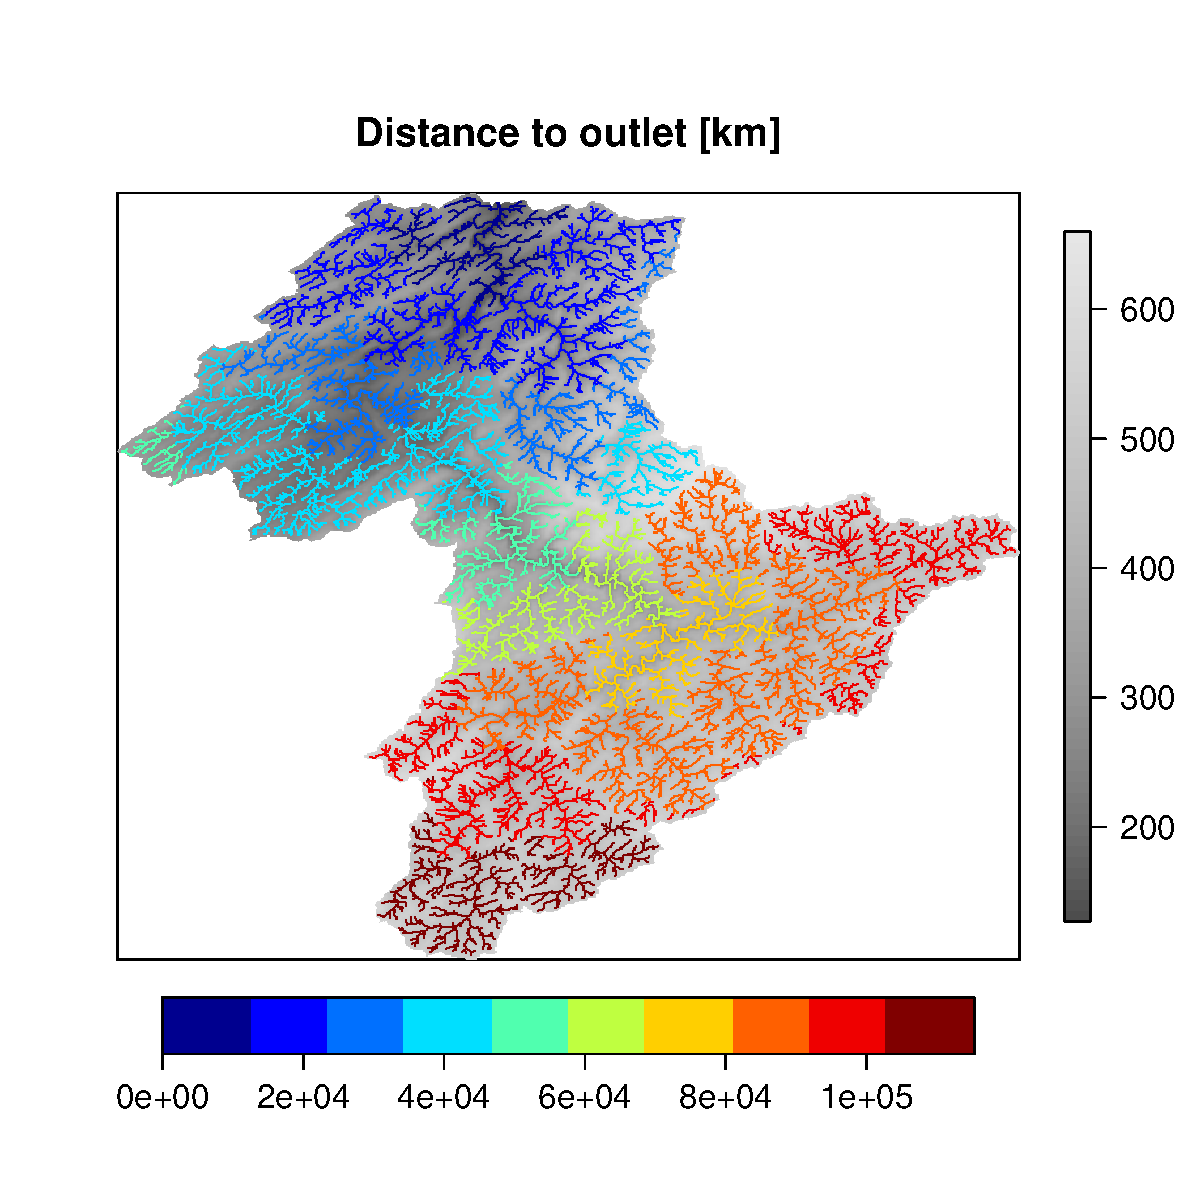
\includegraphics[width=\columnwidth]{Question7.pdf}
115 km\\}
\nQ Plot the average channel elevation versus distance to the outlet. What do the slopes of the curves show?\\
\A{2}{The slope of the channel bed.\\}
\nQ What can you say about the relation between the slopes of the curves and the distance to the outlet?\\
\A{3}{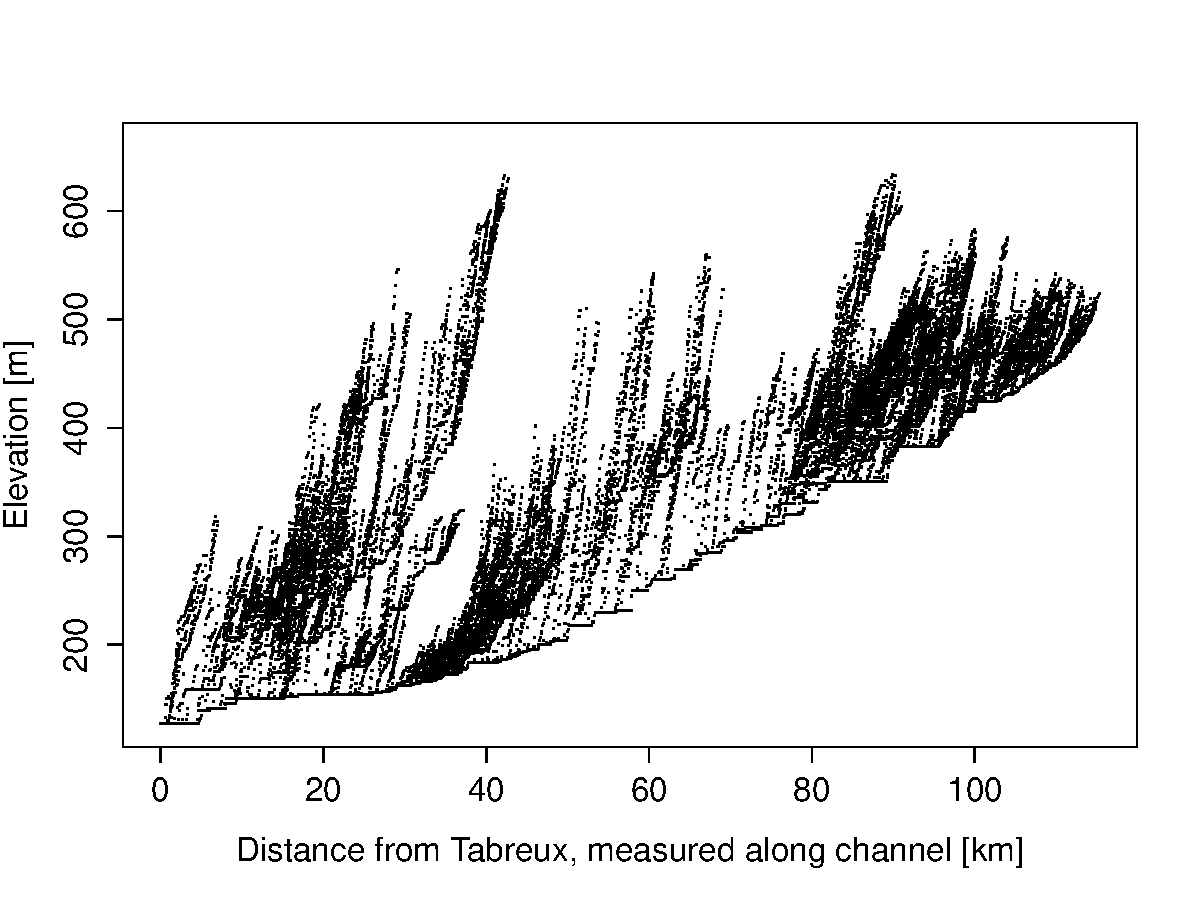
\includegraphics[width=\columnwidth]{Question8.pdf}
Most of the lower order channel links (upstream channel links) have a steeper slope than the higher order ones. The result of this is that close to the sources, the water flows more quickly (when all other factors such as bed roughness and vertical cross-section of the river are considered equal, which is of course not the case as the downstream stretches of river are wider and deeper).\\}
\E


\subsection{Channel width function}
\label{width}
From the channel network you can compute the network width function. This function gives the fraction of channel pixels at a given distance from the outlet. Plot the width function.

\Q Explain the shape of the width function with the shapes of the channel network and catchment.\\
\A{4}{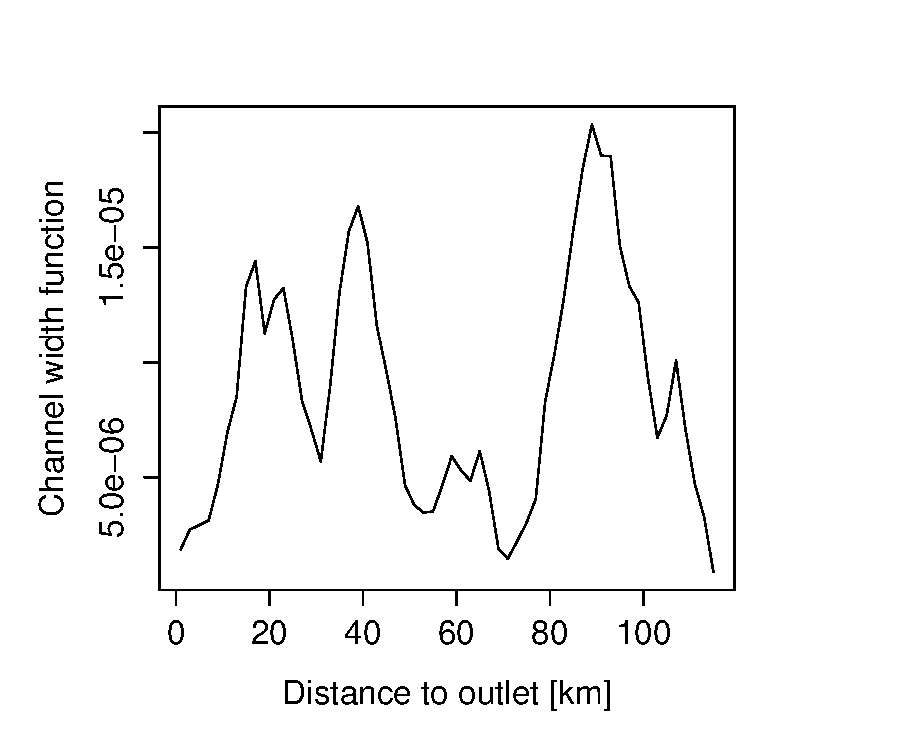
\includegraphics[width=\columnwidth]{Question13.pdf}\\ Close to the outlet (20-40~km) there are many channels, at about 70~km from the outlet there are few channels and between 80 and 100~km from the outlet there are again more channels. From the catchment maps, you can see that the Ourthe catchment has a narrow part in the middle, which causes the low number of links (channel pixels) in the width function.\\}
\E

\subsection{Channel travel time distribution}
The velocity of the water in the river is generally between 0.3 and 3.0~m\,s$^{-1}$. Here a value of 0.8~m\,s$^{-1}$ is assumed for every stretch of river. With the flow velocity you can convert the distance-to-outlet-map into a channel travel time map. 

\Q What can you say about the pattern and variability in flow times and their relation to the shape of the catchment and the channel network?\\
\A{2}{The spatial pattern in the channel travel time map is the same as in the distance-to-outlet-map. To make the travel-time-map, you multiplied the distance-to-outlet at every pixel with a constant, so nothing happened to the spatial distribution.\\}
\E

Different channel velocities lead to different travel time distributions. Compute the maximum and median travel time with different channel velocities ranging from $0.3$ to 3.0~m\,s$^{-1}$ and plot the results (channel velocity on the $x$-axis and travel time on the $y$-axis).

\Q What is the relation between flow velocity and maximum channel travel time?\\
\A{4}{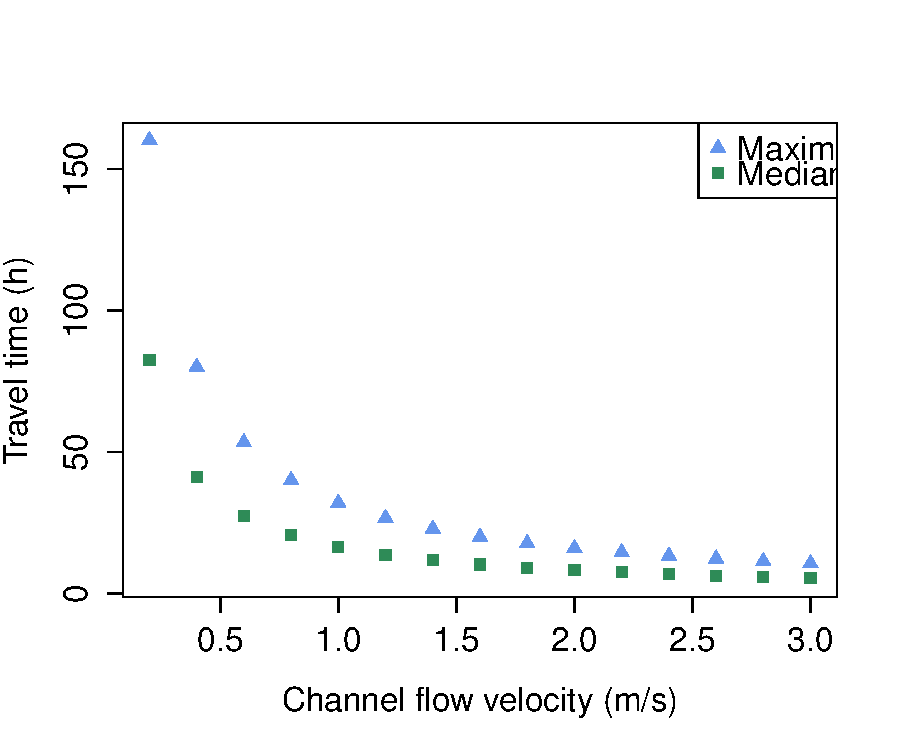
\includegraphics[width=\columnwidth]{Question9.pdf}\\
When the channel velocity doubles, the maximum travel time is halved.\\}
\nQ If all rain would fall on the channel network directly, what do the maximum and median travel time then represent?\\
\A{4}{The time necessary to discharge all or 50\% of the water out of the catchment.\\}
\E

\section{Rainfall-runoff modelling} \label{sec:RRmodeling}
\subsection{Time series}
Before you start modelling, you should get a better feeling of the water balance terms in the Ourthe catchment. The file \verb!PEQ_Ourthe_2002_2003.txt! in the folder \texttt{Data} contains 2~years of basin averaged hourly precipitation [mm\,h$^{-1}$], potential evaporation [mm\,h$^{-1}$] and discharge [m$^{3}$\,s$^{-1}$] data. Use the year 2002 for calibration and Feb.--Dec.~2003 for validation. The discharge data of January~2003 are removed -- you will predict these in the final assignment.

Comparing fluxes is easier when they have the same units. Use the catchment area to convert the discharge to mm\,h$^{-1}$ and plot the time series. To remove the hourly variability, the data can be averaged over monthly periods. This is preprogrammed in the script. In addition, the 10$^\mathrm{th}$ and 90$^\mathrm{th}$ percentiles are computed. 

\Q Look at the seasonal variation to get a rough idea of the dominant fluxes during different seasons.\\
\A{0}{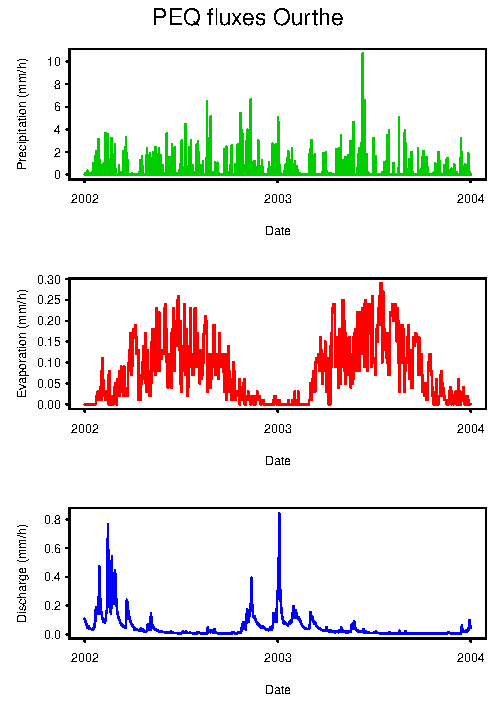
\includegraphics[width=\columnwidth]{Question4.pdf}\\
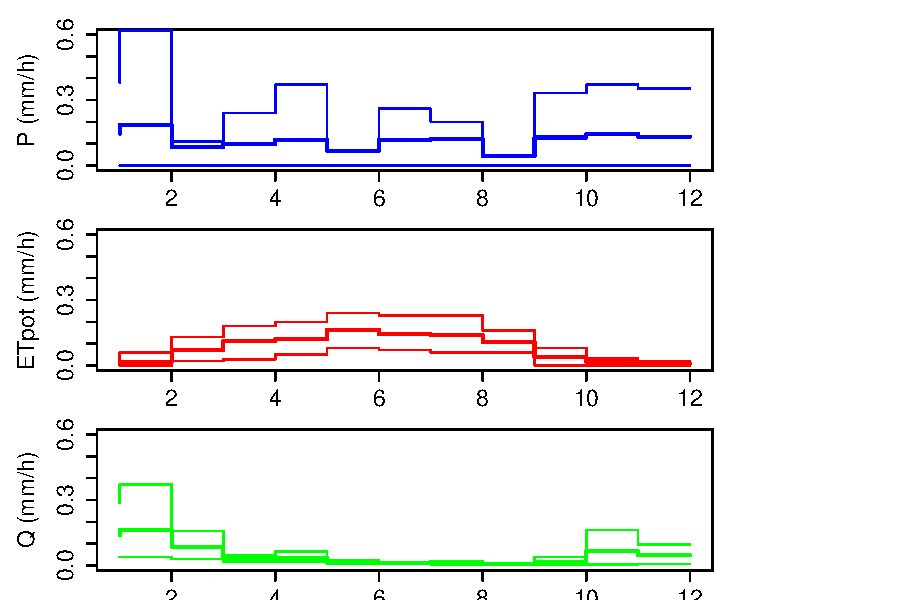
\includegraphics[width=\columnwidth]{Question5.pdf}}
%\newpage
%\Q What can you say about the inter- and intra-monthly variation (inter: between for example January and July; intramonthly: between all January values)?\\
%\A{4}{No clear seasonality can be observed for $P$. $ET_\mathrm{pot}$ shows a sinusoidal curve with maxima in summer. The observed discharge peaks are largest in winter, which is a result of the lower evaporation. For a given month, hourly precipitation data are most variable in both the winter and summer period, which can be related to the type of precipitation (frontal systems and snow in winter vs. frontal systems and convective events in summer).\\ 
%Hourly discharge values vary quite a lot in winter, which is related to the precipitation input variability and the relatively short response time scale (about 1 day) of the Upper Ourthe catchment.\\
%Evapotranspiration varies with magnitude. Maximum evapotranspiration rates are found in summer, when solar radiation and temperature are high. But radiation and temperature vary from day to day (cloudy days), leading to large differences in $ET$.\\} 
%\nQ What are the main differences in water balance terms between the Ourthe and Hupsel Brook catchment that you analysed during practical~2?\\
%\A{4}{The annual precipitation sum is much larger in the Ourthe catchment ($\approx$1000~mm) than in the Hupsel Brook catchment ($\approx$800~mm). $ET_\mathrm{pot}$  is a little higher in the Ourthe catchment because it's further south, leading to more radiation and higher temperatures. Because $P$ is much higher and $ET_\mathrm{pot}$ is more or less equal, $Q$ is much larger in the Ourthe catchment as well .\\}
\E

The models in Chapter~\ref{sec:RRmodeling} need input, but cannot deal with negative input ($ET>P$), because they do not contain stores from which water can be removed (they use transfer functions instead of reservoirs). You could just use $P$ as input, but of course part of the precipitation evaporates. As a quick fix, a factor $f$ is introduced to close the water balance over 2002 to account for evapotranspiration: \[f \cdot \Sigma P - \Sigma Q=0\ .\] Hourly values of effective precipitation are computed as
\[P_\mathrm{eff} = f \cdot P\ .\] 

\subsection{Channel travel time distribution model} \label{sec:tt}
From the channel width function in section~\ref{width} you can make a simple rainfall-runoff model. In this model you assume that all precipitation enters the channel network directly. 
 
The function \verb!Q_geomorph_channel! converts the width function to a travel time distribution model with a convolution integral. Try to understand the different aspects of this function (look in the file \verb!Q_geomorph_channel.R!). 

Run this function with the effective precipitation time series and flow velocity parameter.
 
\Q How does the simulated discharge compare to the observed discharge? What happens if you change the velocity?\\
\A{3}{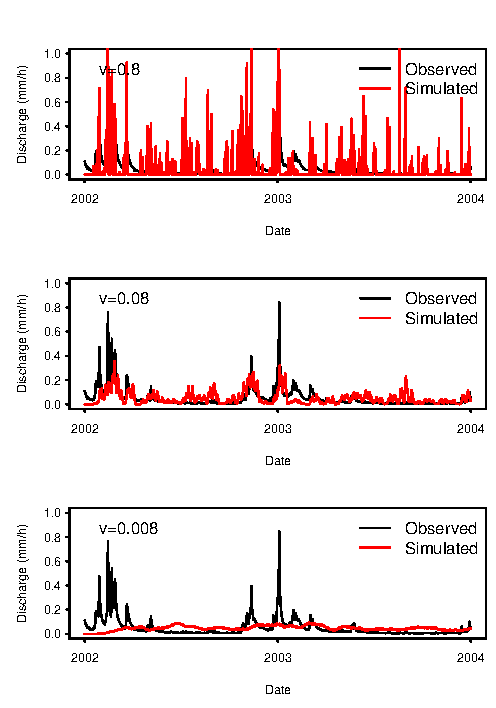
\includegraphics[width=\columnwidth]{Question14.pdf}
With a velocity of 0.8 m~s$^{-1}$ the response is too flashy, while for very slow values (0.008 m~s$^{-1}$) there is no clear response of runoff to rainfall.\\}
\E


\subsection{Hillslope width function}
Of course, the assumption that all precipitation immediately enters the channel network is not valid: the simulated discharge response is too fast. This illustrates that the response of a catchment is not only characterized by the channel network but also by the soil, slope and vegetation on the hillslopes.

Compute for each pixel the distance to the nearest channel, plot the map and make a histogram: the hillslope width function.\\
\A{0}{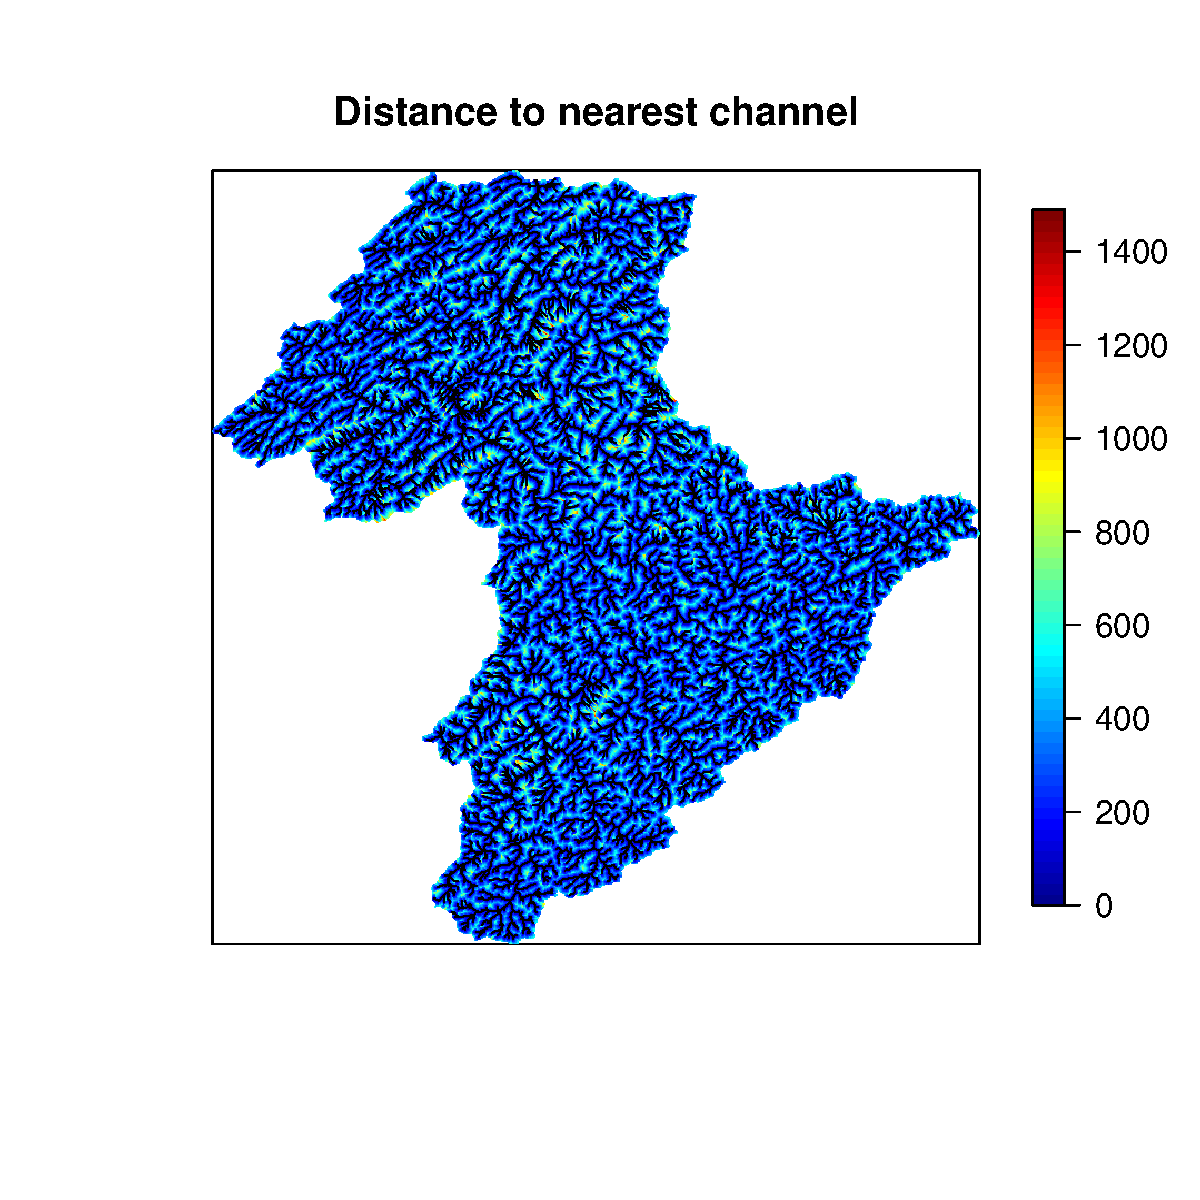
\includegraphics[width=\columnwidth]{Question15.pdf}\\}
\Q What is the average distance to the channel?\\
\A{1}{250~m.\\}
\nQ How does the average distance to the channel compare to the average hillslope length you computed in Section~\ref{sec:dd}?\\
\A{2}{They compare quite well.\\}
\nQ What information does this width function give?\\
\A{4}{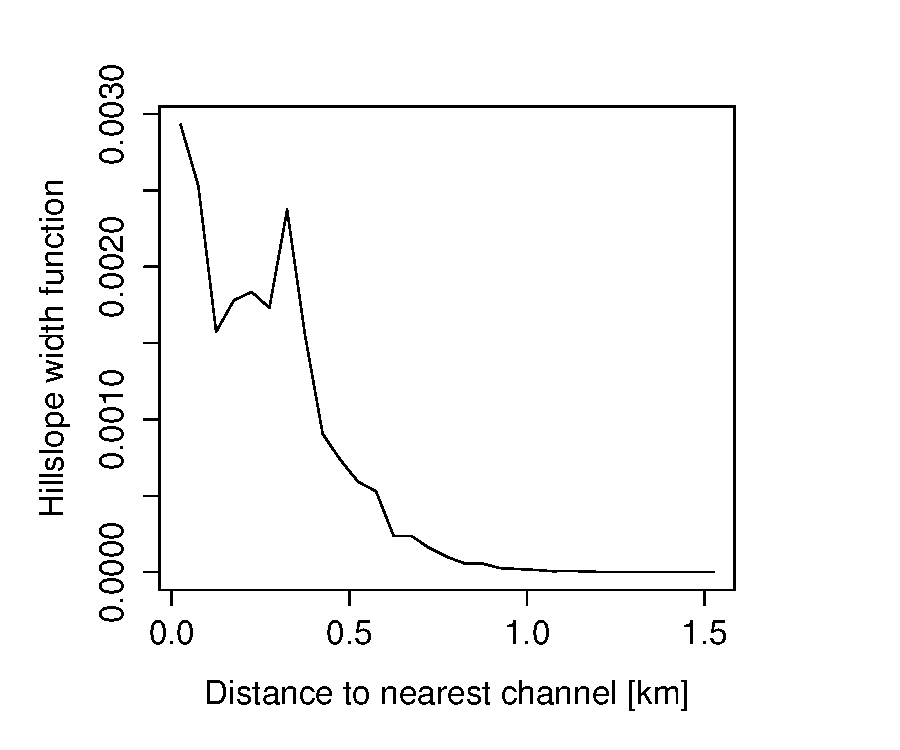
\includegraphics[width=\columnwidth]{Question15_2.pdf}\\
Most pixels are close to a channel and the number of pixels at a certain distance from a channel decreases with that distance to the channel. There are few pixels more than 100~m away from the nearest channel.\\}
\E

\subsection{Channel and hillslope travel time distribution model}
A catchment's travel time distribution is determined by the time a water droplet spends in both the hillslope and the channel network. You already computed the channel travel time distribution from the channel width function (Sec.~\ref{sec:tt}). In the same way, you can make a hillslope travel time distribution from the histogram of the distances to the nearest channel. Just as in the channel, we assume that the flow velocity in the hillslope is constant.

\Q Why is the assumption of a constant (no variation in time) flow velocity in the hillslope not realistic?\\
\A{4}{Water travels overland, through macropores and the unsaturated and saturated zone matrix. Between these flow routes, velocity can easily differ by a factor 100. The distribution of water over these flowpaths varies temporally\\}
\E

The functions \verb!Q_geomorph_hillslope! and \verb!Q_hillslope_parts! have a similar set-up as the previously used function \verb!Q_geomorph_channel!. As a first estimate, the effective\footnote{The word effective is added because the actual flow velocity of the water particles through the soil is much slower than the response caused by pressure changes.} velocity in the hillslope is assumed to be 0.1~m\,s$^{-1}$ and the channel network velocity 0.8~m\,s$^{-1}$.

\Q During which part of the year do the simulated discharge peaks fit the observed ones well? Why?\\
\A{4}{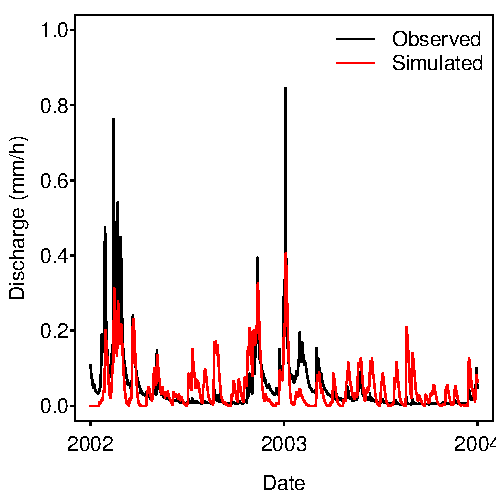
\includegraphics[width=\columnwidth]{Question16.pdf}
The simulated model performs best during the winter period, but, because the amount of evaporation was assumed to a fixed percentage of the amount of precipitation, even during the winter year the response is underestimated.\\}
\nQ What happens to the baseflow? Why?\\
\A{4}{Baseflow results from very slow runoff processes. Because only one value for the flow through the hillslope is taken into account, baseflow is not simulated. In general, it can be expected that baseflow results from much smaller velocities in the hillslope than modelled here.\\}
\E

Try different values for the effective hillslope velocity.

\Q Which values for the effective hillslope velocity yield good results in the winter period and which in the summer?\\
\A{2}{Many values possible.\\}
\nQ You probably found that in winter the hillslope velocity is higher than in in summer. Explain this with the dominant processes that occur during winter.\\
\A{4}{As mentioned in the previous question, this model did not take the yearly behaviour in the observed evaporation into account. Therefore, the effective precipitation in the winter (summer) period is too small (large). For very small hillslope velocity values, the summer response is fairly well simulated.\\}
\E

\subsection{Flow routes}
The route a water droplet takes through the hillslope to the channel depends on many factors, such as soil type, presence of macropores, vegetation and catchment wetness. Because many of these factors change during the year, the flow routes change, and therefore the travel times change.

Make the model a bit more complex by assuming that the hillslope can be modelled with three different hillslope velocity values, $v=10^{-3}$, $v=10^{-5}$ and $v=10^{-7}~\mathrm{m\,s^{-1}}$, indicating the fast, intermediate and slow hillslope response. Run the model with the defined fractions for fast, medium and slow response velocities.

\Q Play around with the fractions of the different velocities. Which fractions did you get for which part of the year? \\
\A{2}{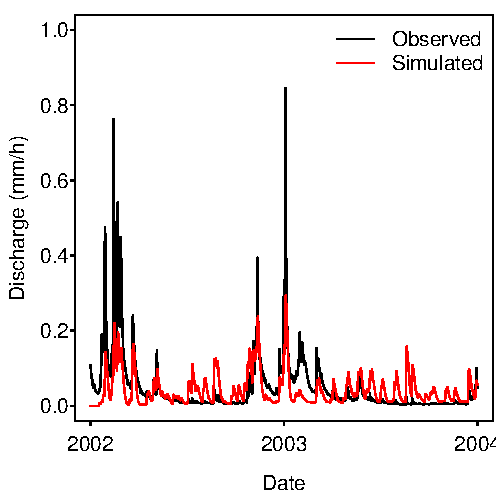
\includegraphics[width=\columnwidth]{Question17.pdf} Many answers possible\\.}
\nQ For which part of the year were you able to obtain proper discharge estimates?\\
\A{2}{Probably in winter.\\}
\E

\vspace{-5mm}
\section{TOPMODEL} \label{sec:topmodel}
As you probably noticed, the simple model was only able to simulate a proper response behaviour for some events. It is very difficult to simulate the hydrological response of a catchment with a few fixed velocities. It is impossible to grasp the temporal variations in the complex hydrological interactions between vegetation and the unsaturated and saturated zones using this simple approach. 

The next step is to use a more complex (but still relatively simple) hydrological model: TOPMODEL. TOPMODEL is a well-known model based on the topographic properties of the catchment. 

\subsection{Topographic index}
The main assumption behind TOPMODEL is that the response behaviour of a given pixel can be estimated by its topographic index value $\lambda$:
\[ \lambda = \ln \left( \frac{a}{\tan \beta}\right)\ ,\]
where $a$ is the upstream area per unit contour length (pixel length) [m] and $\beta$ the local slope [$^\circ$]. More information on TOPMODEL is given in the reader.

Use the script to compute and plot the topographic index for each pixel.

%\newpage
\Q How are the topographic indices distributed?\\
\A{4}{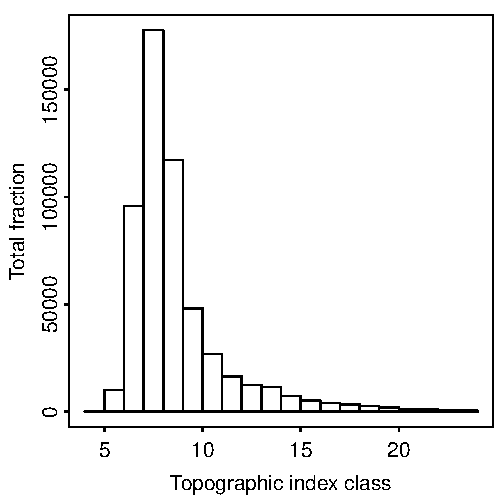
\includegraphics[width=\columnwidth]{Question18.pdf} 
Most cells have a small topographic index value, indication either a small upstream area or large local slope. Both of these characteristics can expected to be observed further away from the channel sections.\\}
\E

\subsection{Running TOPMODEL}
To run TOPMODEL, you need to specify 5~parameters and 2~initial conditions. 
%TOPMODEL has 5 parameters of which the values are different for each catchment and can be found by model calibration (also called parameter estimation or optimization). Calibration is often difficult because different parameter sets may lead to more or less equally good results. 
TOPMODEL has already been calibrated for the Ourthe catchment and 20~parameter sets are given in \verb!TOPMODEL_Parameters.dat!. The initial conditions are the unsaturated zone deficit (\texttt{Dbar}) and  root zone deficit (\texttt{Drzone}), both effective catchment values.

First, use only the first parameter set (first row in \verb!TOPMODEL_Parameters.dat!). Run TOPMODEL and simulate the discharge response. Choose the period yourself. 

\Q Describe the performance of the model. When did the model succeed and when and how did it fail?\\
\A{3}{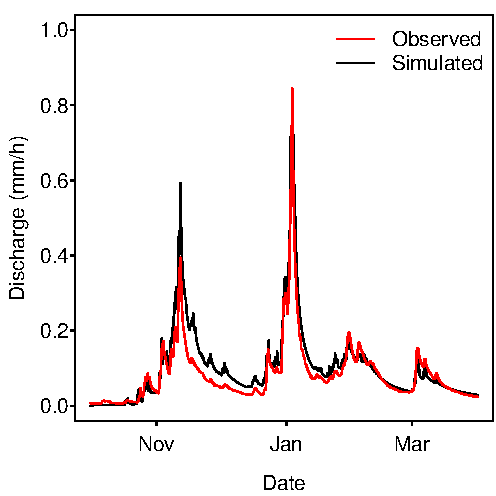
\includegraphics[width=\columnwidth]{Question19.pdf}
TOPMODEL is quite well able to simulate the hydrologic response of the Ourthe catchment. However looking more closely, the simulated discharge is too large (small) at the beginning (end) of the winter. These latter properties are a consequence of the assumption of a fixed upstream recharge area, which is practice varies over time.\\}
\E

\subsection{Effect of parameters}
To analyze the effect of uncertainty in the parameter values, run the model with all 20 parameter sets and make an ensemble of the simulations. This may take a few minutes. 

\Q When is the parameter uncertainty large? In other words, when is the spread of the grey lines, caused by different parameter sets, large?\\
\A{4}{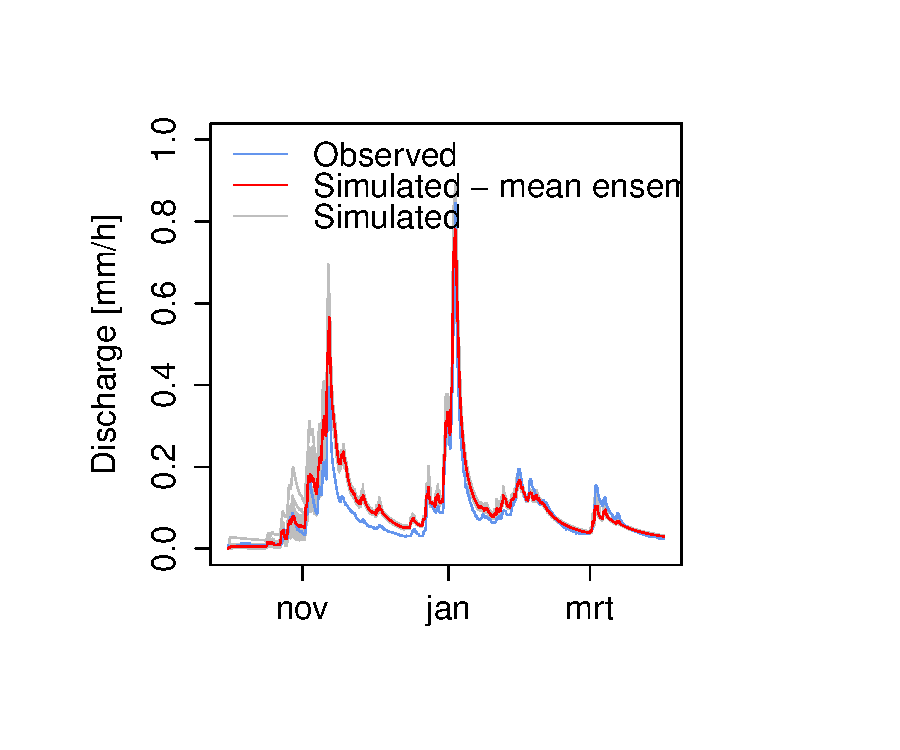
\includegraphics[width=\columnwidth]{Question20.pdf}\\
The parameter uncertainty is especially large during the first rising limb (Oct-Nov).\\}
\E

\subsection{Effect of initial conditions}
The results show that it is especially difficult to simulate the response of the Ourthe for the first main runoff peak in November~2002. This is caused by a wrong estimation of the initial storage, given by \texttt{Dbar} and \texttt{Drzone}. 

Change the values of \texttt{Dbar} and \texttt{Drzone} and run the model again.

\Q What is the effect of the initial conditions?\\
\A{4}{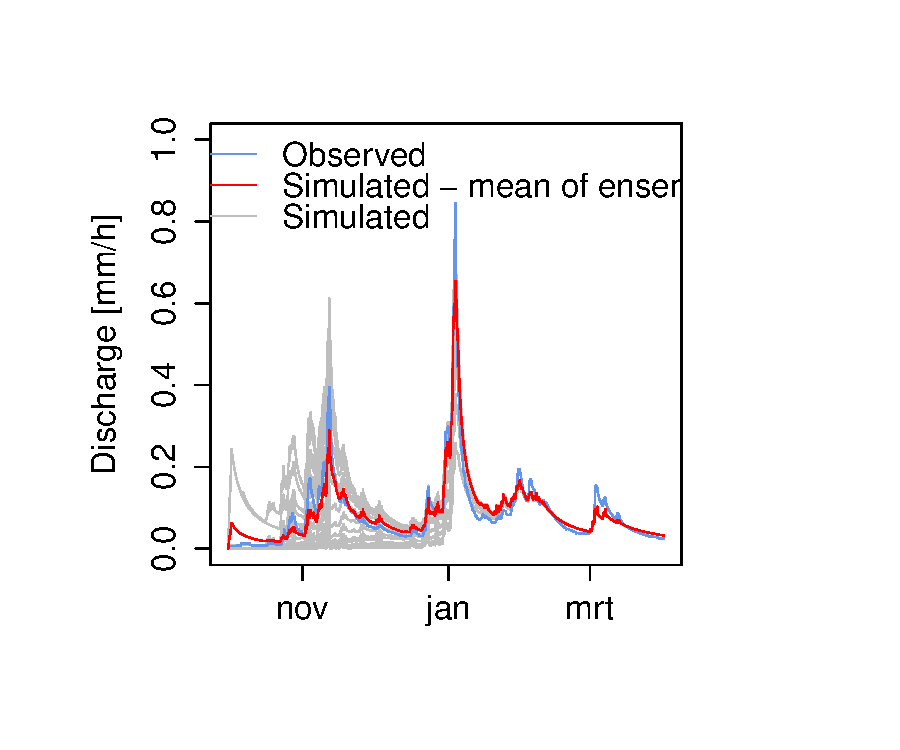
\includegraphics[width=\columnwidth]{Question21.pdf} 
The initial values determine how ``wet" the catchment is at the start of the modelling period. When you assume that the catchment is wetter than it really is, you will overestimate the discharge response in the beginning of the period. After a few months, the saturated zone and rootzone deficit will go down to the ``real" values, because when you start too wet, you will get more discharge and you will get a sort of equilibrium value (Dbar and Drzone have gone up and down again and the influence of the initial values becomes less important).\\
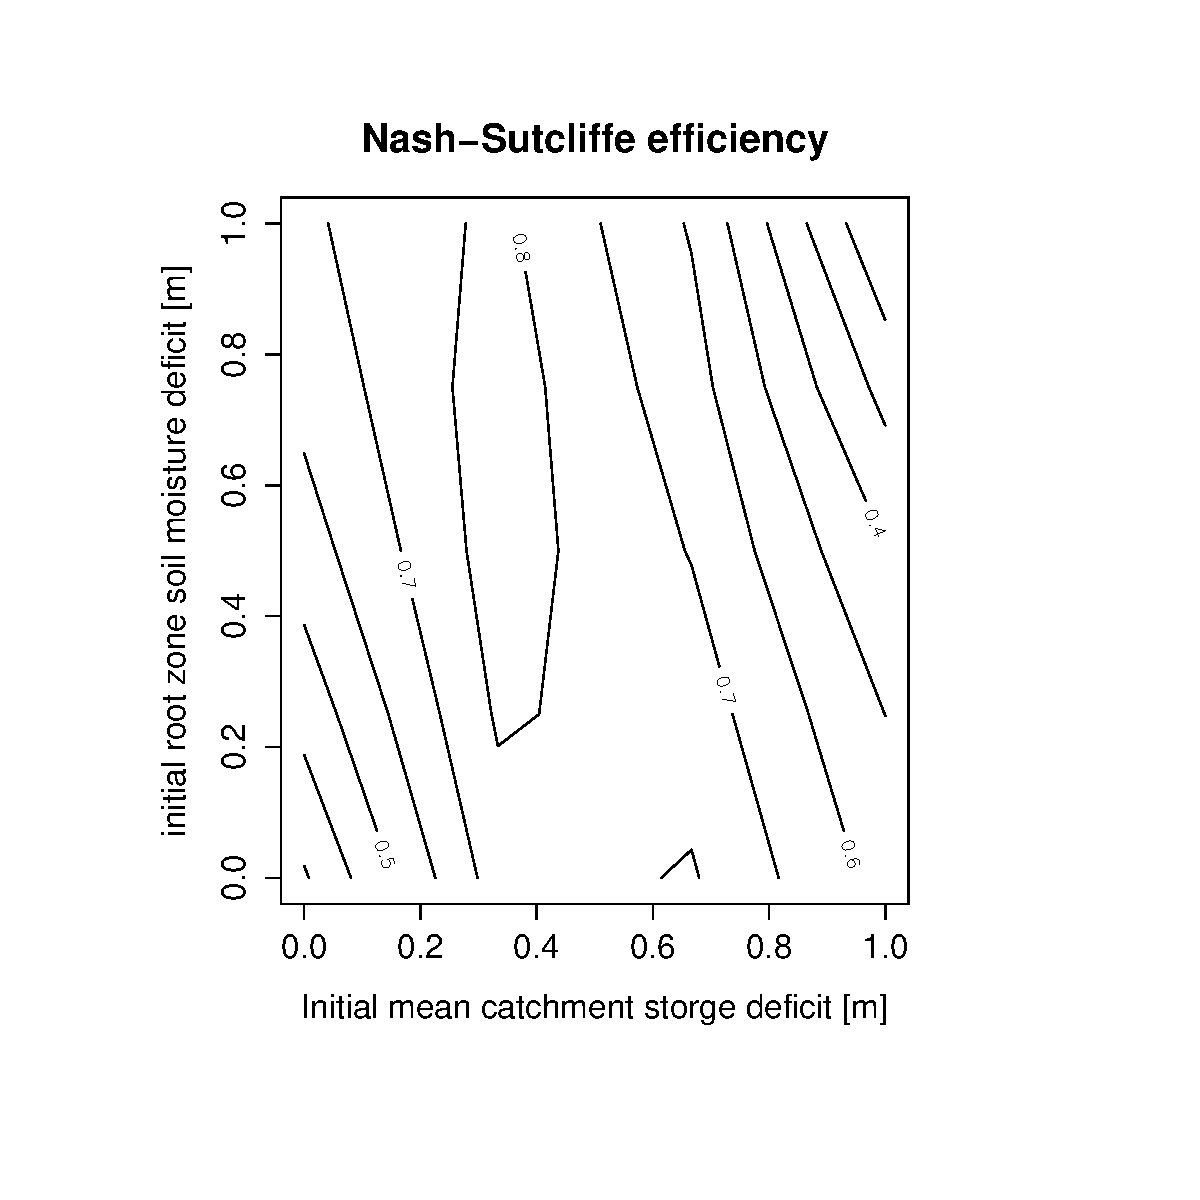
\includegraphics[width=\columnwidth]{Question22.pdf} 
The best results are obtained from either large (small) values of the saturated zone deficit (Dbar) and small (large) the root zone deficit (Drzone). In case both would have a really large (small) deficit value, the initial storage of the Ourthe would be under (over) estimated.\\}
\E 

Some models use a warming-up period to compensate for bad initial conditions. For example, when you want to forecast discharge from April to September, you may start the simulations in March and neglect the output of the first month. 

\Q How long would you advise the warming-up period to be for TOPMODEL in the Ourthe catchment and why?\\
\A{4}{The effect of the initial conditions is visible for about 3.5 months. After this, the simulations with different initial conditions are similar.\\} 
\nQ  What is the relation between \texttt{Dbar} and \texttt{Drzone}?\\ 
\A{4}{In reality, there usually is much water in the root zone when the saturated zone is full. In the model, when you increase both, you will overestimate discharge and when you decrease both you underestimate. In the middle there is an area where you can exchange Dbar and Drzone: you can increase Dbar a little and decrease Drzone to get the same total storage leading to more or less the same discharge response and therefore the same Nash-Sutcliffe efficiency.\\}
\E

\subsection{Final assignment}
Predict the discharge peak in January~2003 using TOPMODEL. Run TOPMODEL with different settings. You can change (1) the warming-up period, (2) parameter sets and (3) initial conditions. Collect the computed discharge from different runs as columns in a matrix to get an ensemble of forecasts, which you can plot and analyse. Follow the instructions in the script.

Compute the 25th, 50th and 75th percentile of the ensemble and cut out the values of January (so 3~time series with 744~values). Save the output as a CSV file in your working directory. Open the file in Excel, copy and paste it in Google Sheets before 13:00. We will discuss the results at 13:05.


\end{PC_prac_environment}
\end{document}